\subsection*{Teil B: Kreise (20 Minuten)}

\begin{enumerate}[resume, label=\arabic*.]
    \item \textbf{Zeichne mit dem Zirkel:}
    \begin{enumerate}[label=\alph*)]
        \item Einen Kreis mit Radius $r = 3$ cm

        \vspace{5cm}

        \item Einen Kreis mit Durchmesser $d = 5$ cm
        \textit{Hinweis: Wie groß ist der Radius?}

        \vspace{5cm}
    \end{enumerate}

    \vspace{0.5cm}

    \item \textbf{Beschrifte die Teile des Kreises:}

    \begin{center}
        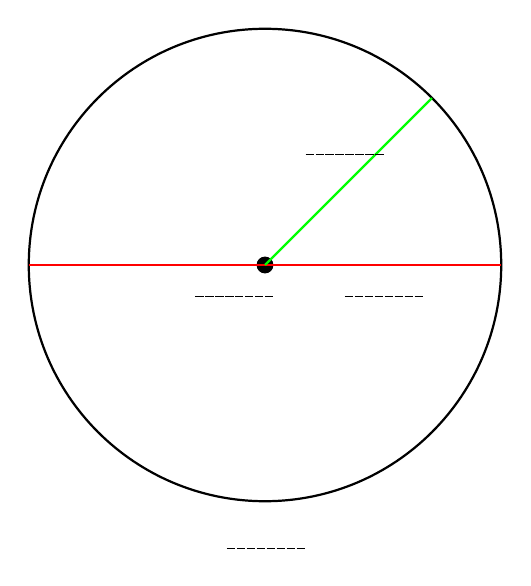
\begin{tikzpicture}[scale=2]
            \draw[thick] (0,0) circle (1.5cm);
            \draw[fill=black] (0,0) circle (0.05cm);
            \draw[thick,blue] (0,0) -- (1.5,0);
            \draw[thick,red] (-1.5,0) -- (1.5,0);
            \draw[thick,green] (0,0) -- (1.06,1.06);
            \node at (0.75,-0.2) {\_\_\_\_\_\_\_\_};
            \node at (0,-1.8) {\_\_\_\_\_\_\_\_};
            \node at (0.5,0.7) {\_\_\_\_\_\_\_\_};
            \node at (-0.2,-0.2) {\_\_\_\_\_\_\_\_};
        \end{tikzpicture}
    \end{center}

    \textit{Wörter zum Einsetzen: Mittelpunkt, Radius, Durchmesser, Kreislinie}

    \vspace{0.5cm}

    \item \textbf{Berechne:}
    \begin{enumerate}[label=\alph*)]
        \item $r = 4$ cm, wie groß ist der Durchmesser? 

        Rechnung: $d = 2 \cdot r = 2 \cdot 4$ cm = \underline{\hspace{3cm}}

        \item $d = 10$ cm, wie groß ist der Radius? 

        Rechnung: $r = d : 2 = 10$ cm $: 2$ = \underline{\hspace{3cm}}
    \end{enumerate}
\end{enumerate}